%\chapter{Manuál}

%\chapter{Konfigurační soubor}

%\chapter{RelaxNG Schéma konfiguračního souboru}

\chapter{Ukázka hardwarových zařízení} \label{appendices-hardware-images}
V~této kapitole jsou ukázána některá hardwarová zařízení používaná v~rámci této práce. Popis firmwarů pro tato zařízení je možné nalézt v~kapitole \ref{hardware-implementation}.

\begin{figure}[H]
  \begin{minipage}[b]{0.4\textwidth}
    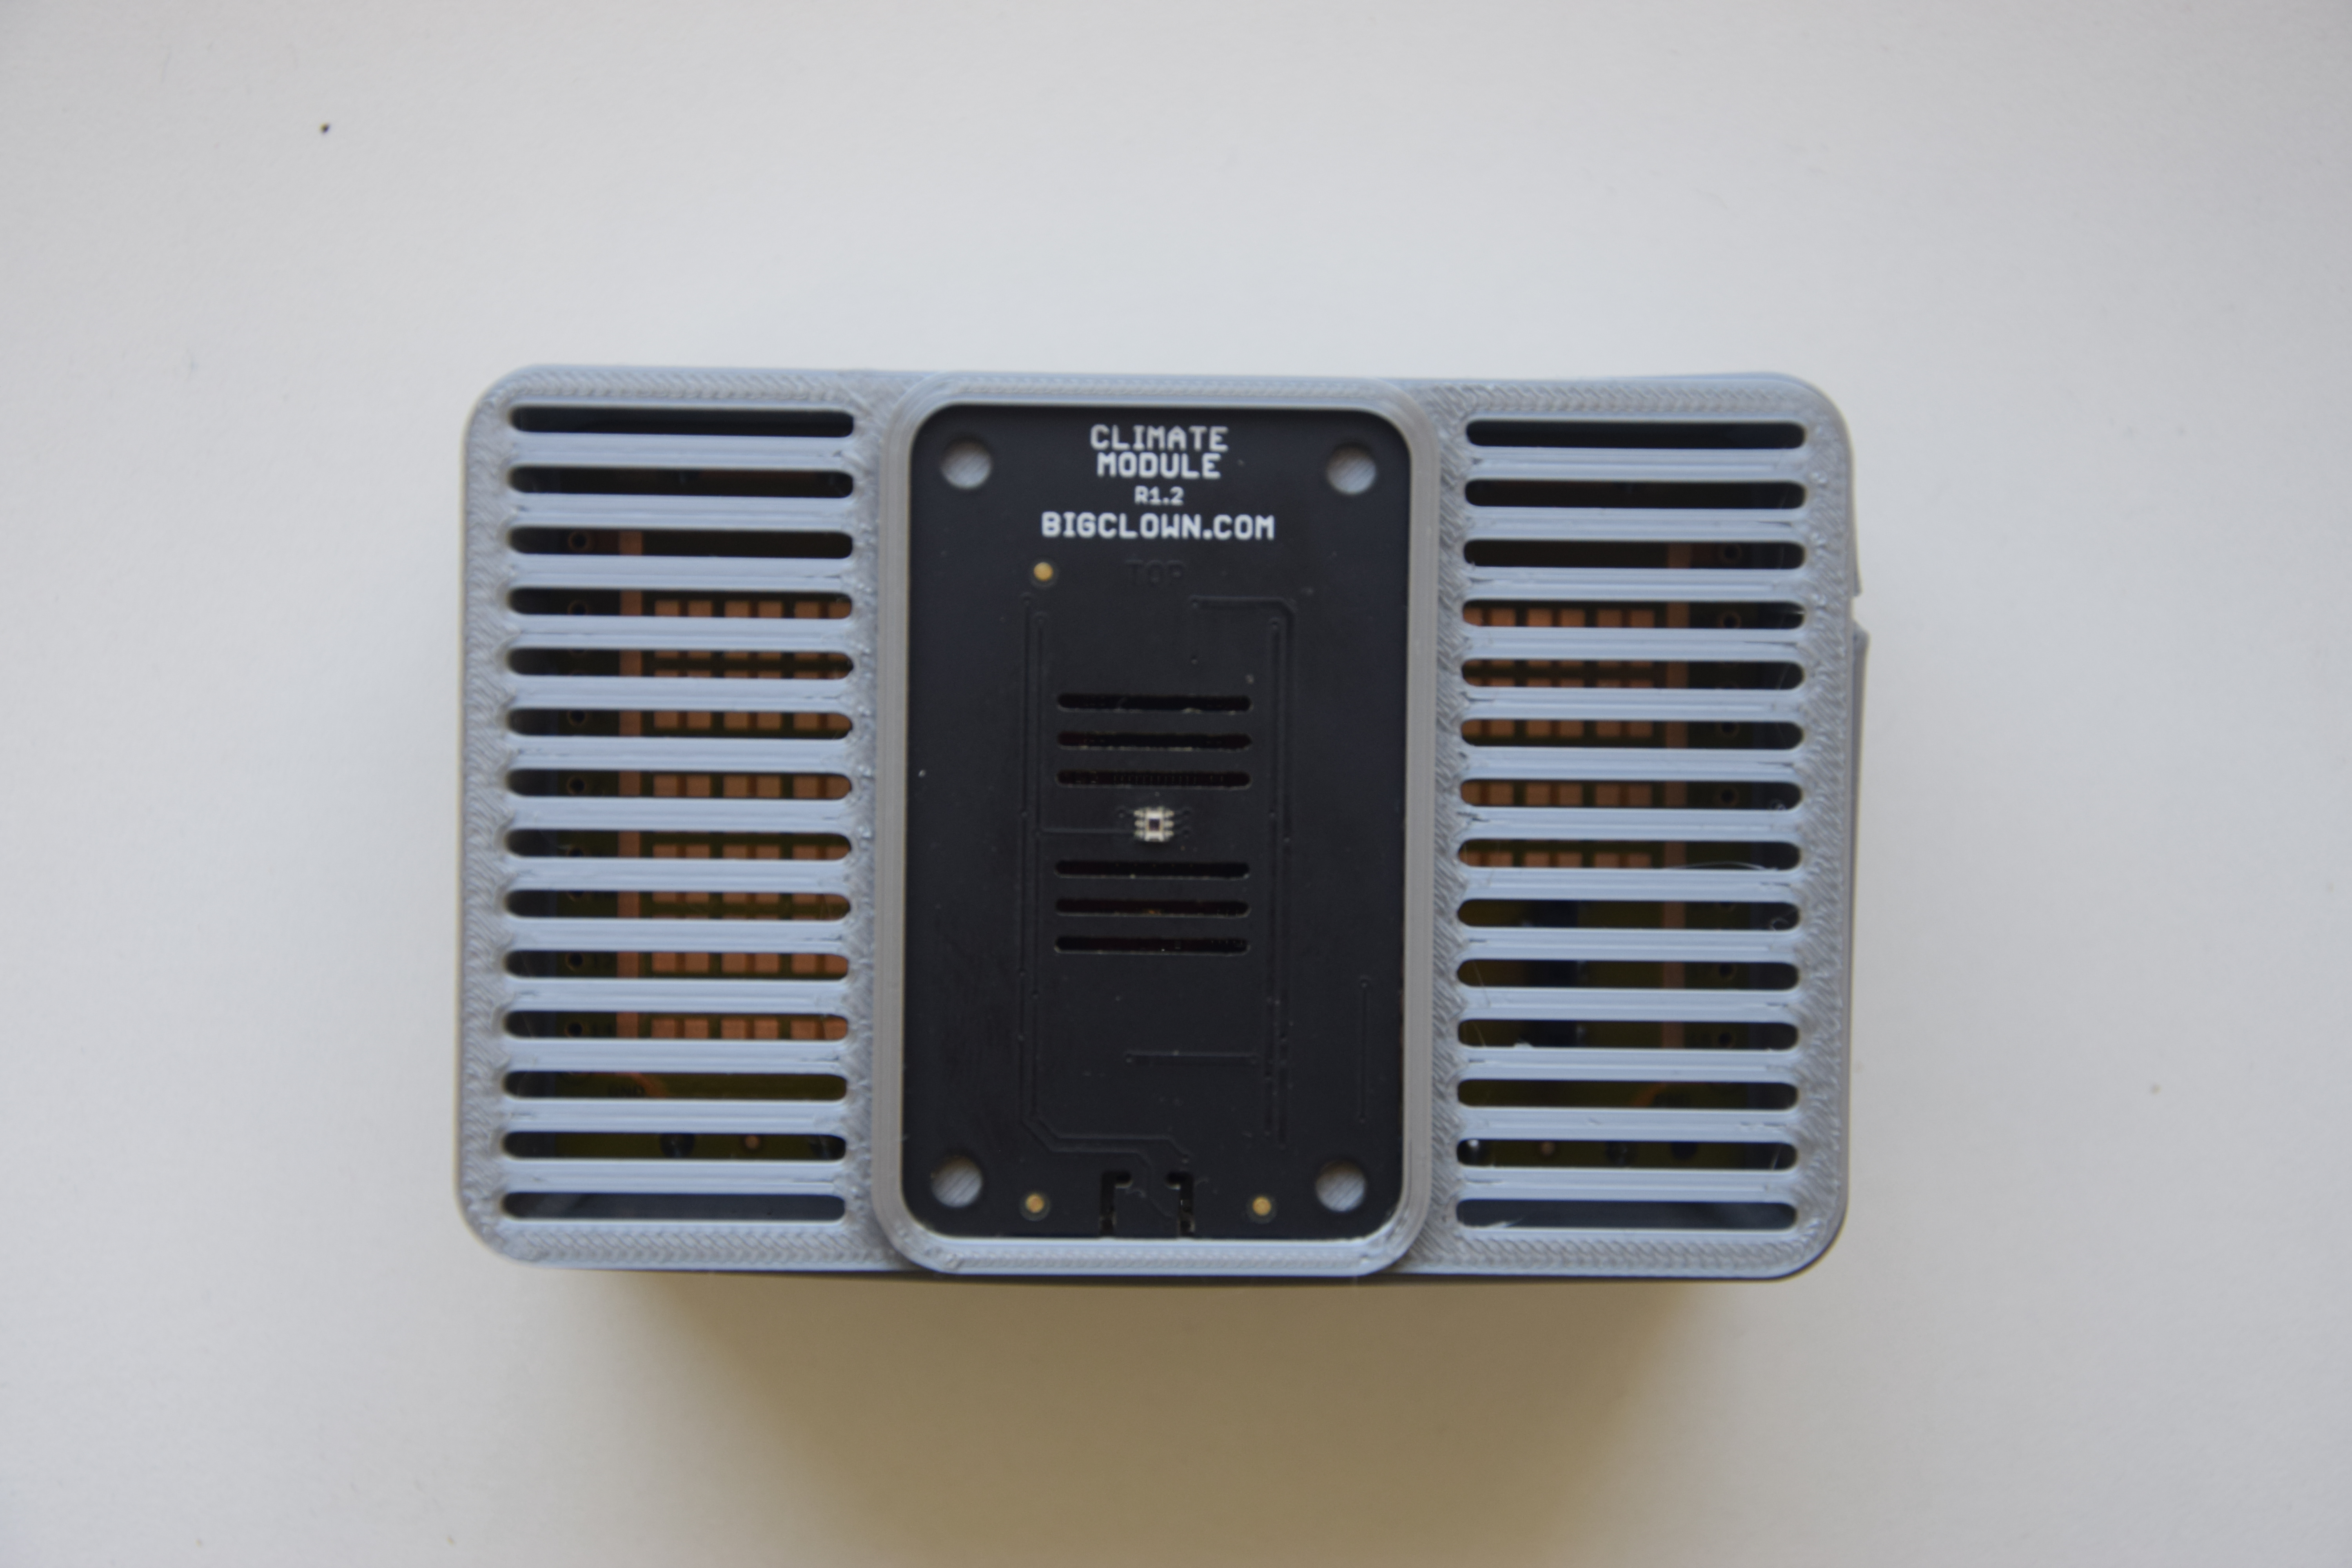
\includegraphics[width=\textwidth]{obrazky-figures/hardwarePhotos/climateMonitor.JPG}
    \caption{Monitor klimatických podmínek pro indoor či outdoor. Foto autor}
    \label{completeClimateMonitor}
  \end{minipage}
  \hfill
  \begin{minipage}[b]{0.4\textwidth}
    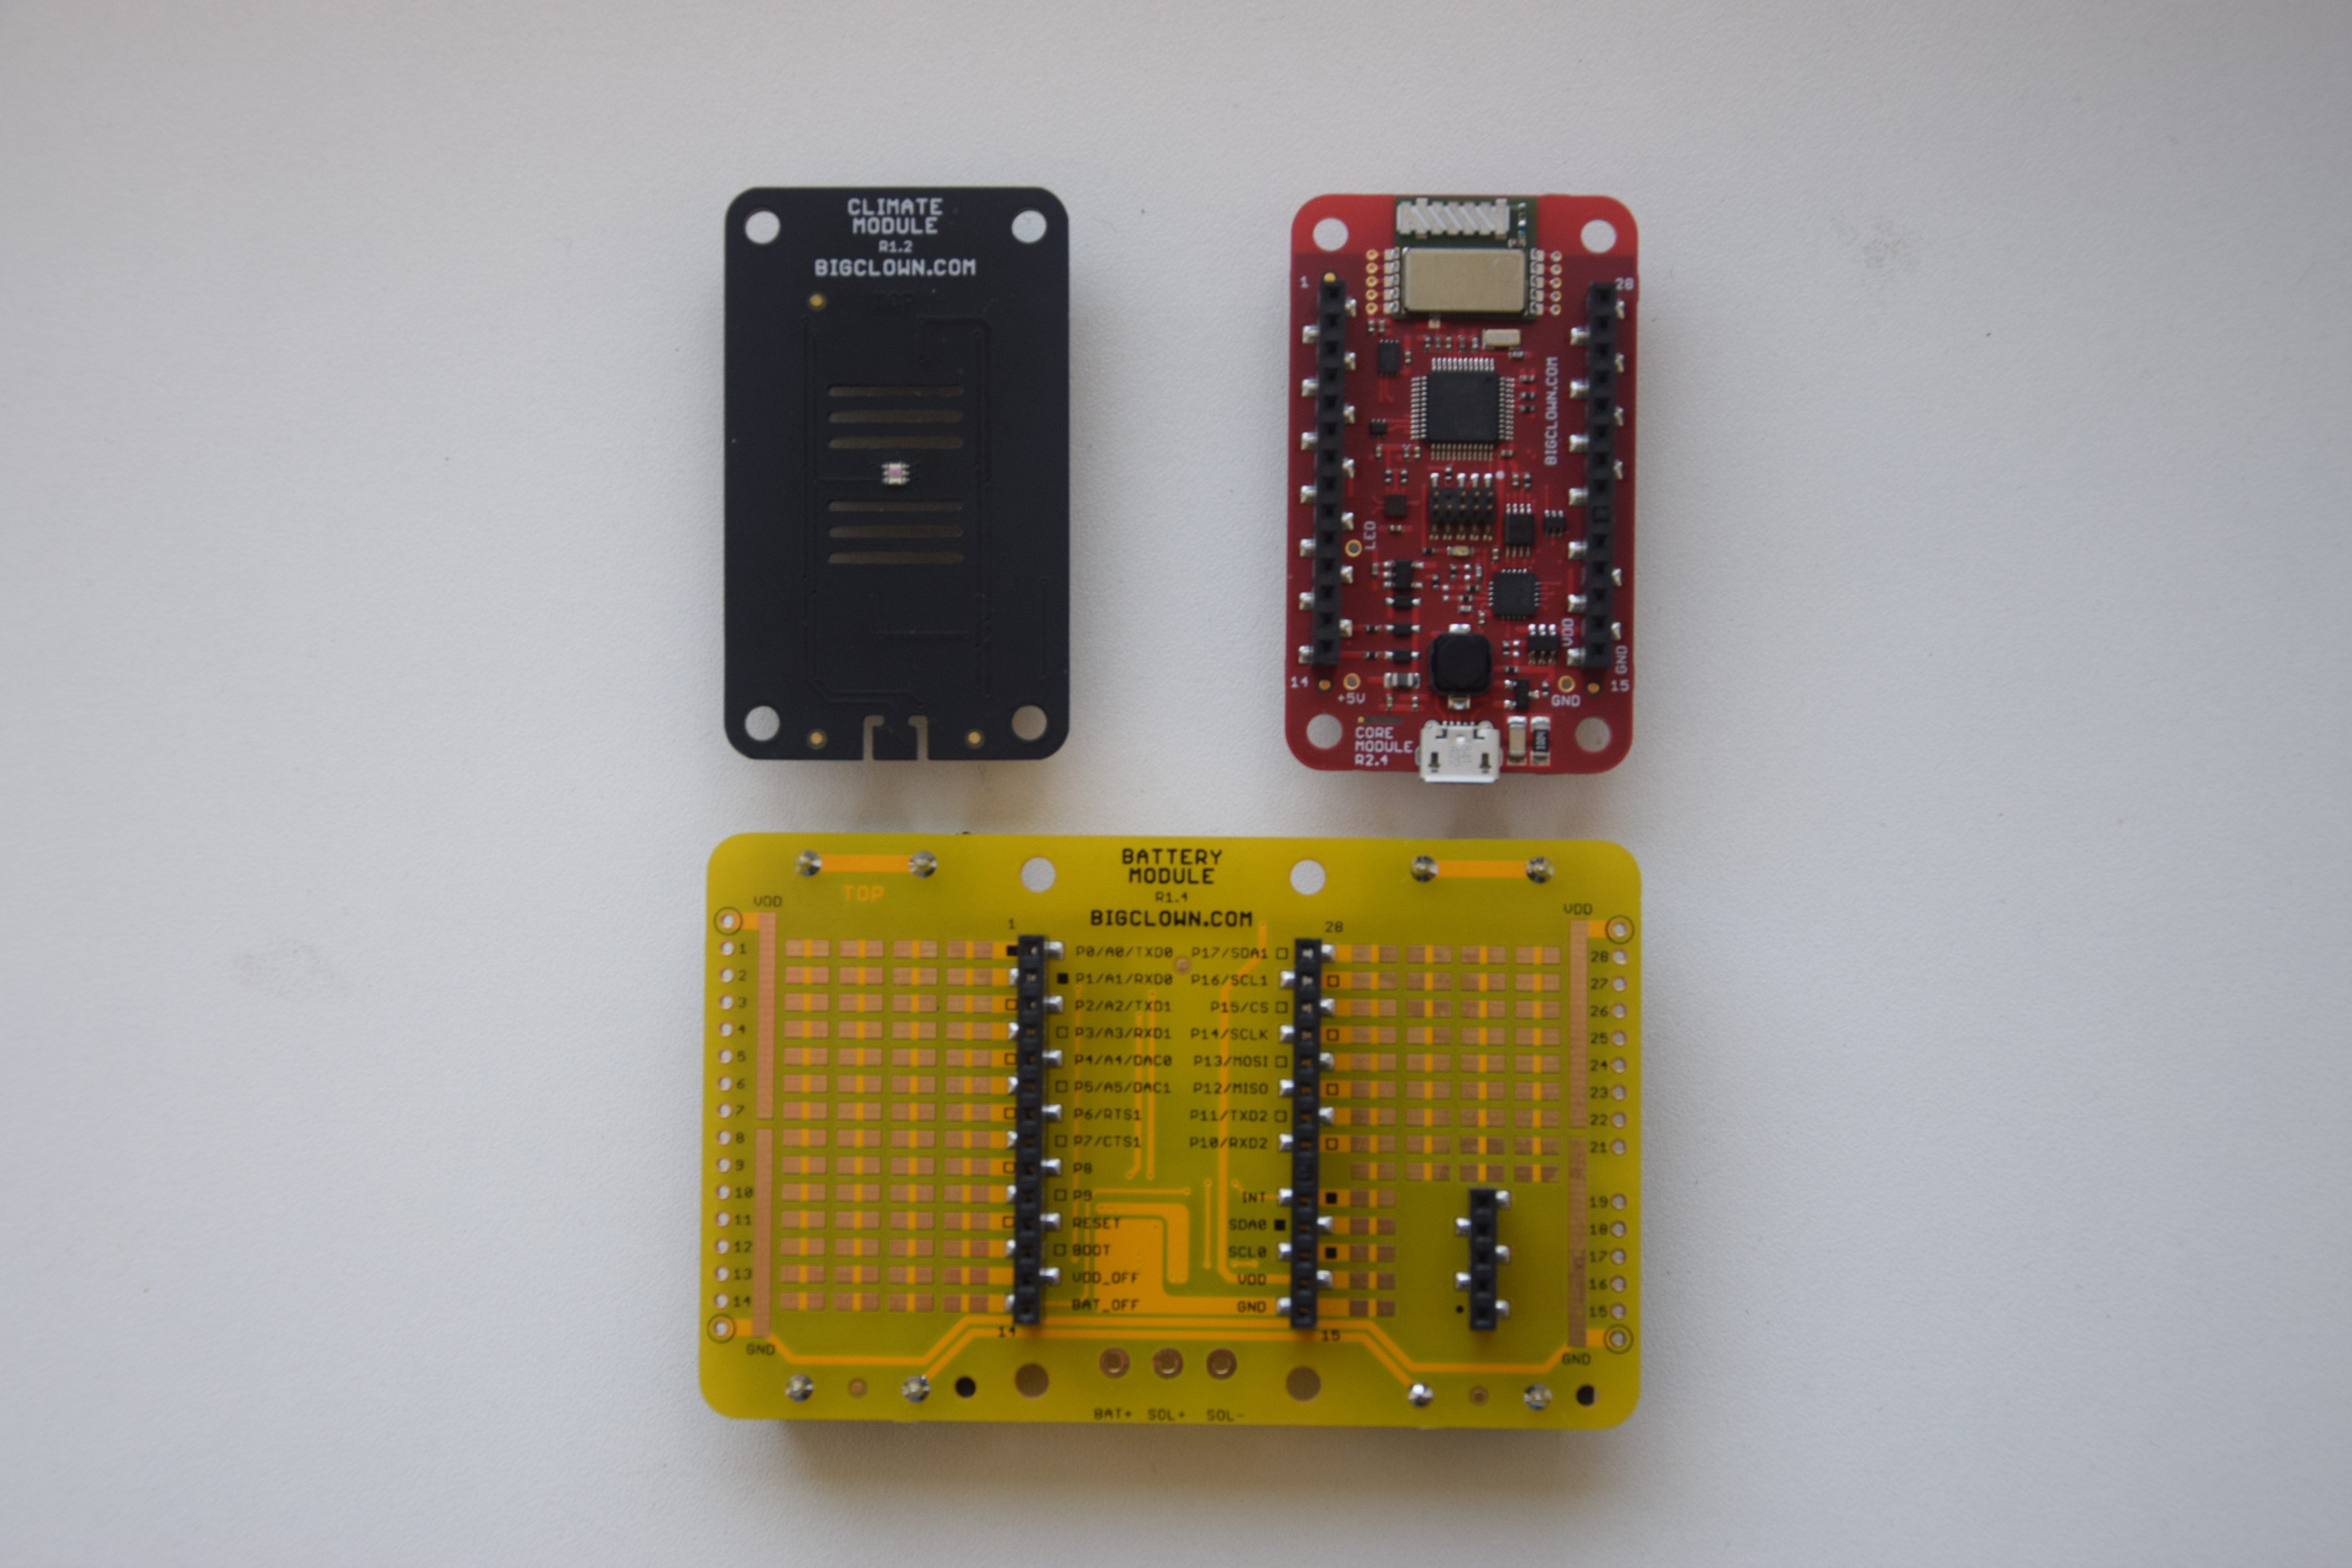
\includegraphics[width=\textwidth]{obrazky-figures/hardwarePhotos/climateMonitorParts.JPG}
    \caption{Stejné zařízení rozložené na jednotlivé moduly. Foto autor}
    \label{disasembeledClimateMonitor}
  \end{minipage}
\end{figure}

Na obrázku \ref{disasembeledClimateMonitor} je vidět rozložené zařízení. Žlutý modul je napájecí bateriový modul, červený obsahuje samotný mikroprocesor a ovládá celé zařízení a černý modul se stará o~měření klimatických podmínek. Toto zařízení je složeno a umístěno do vytisknuté krabičky na Obrázku \ref{completeClimateMonitor}.

\begin{figure}[H]
  \begin{minipage}[b]{0.4\textwidth}
    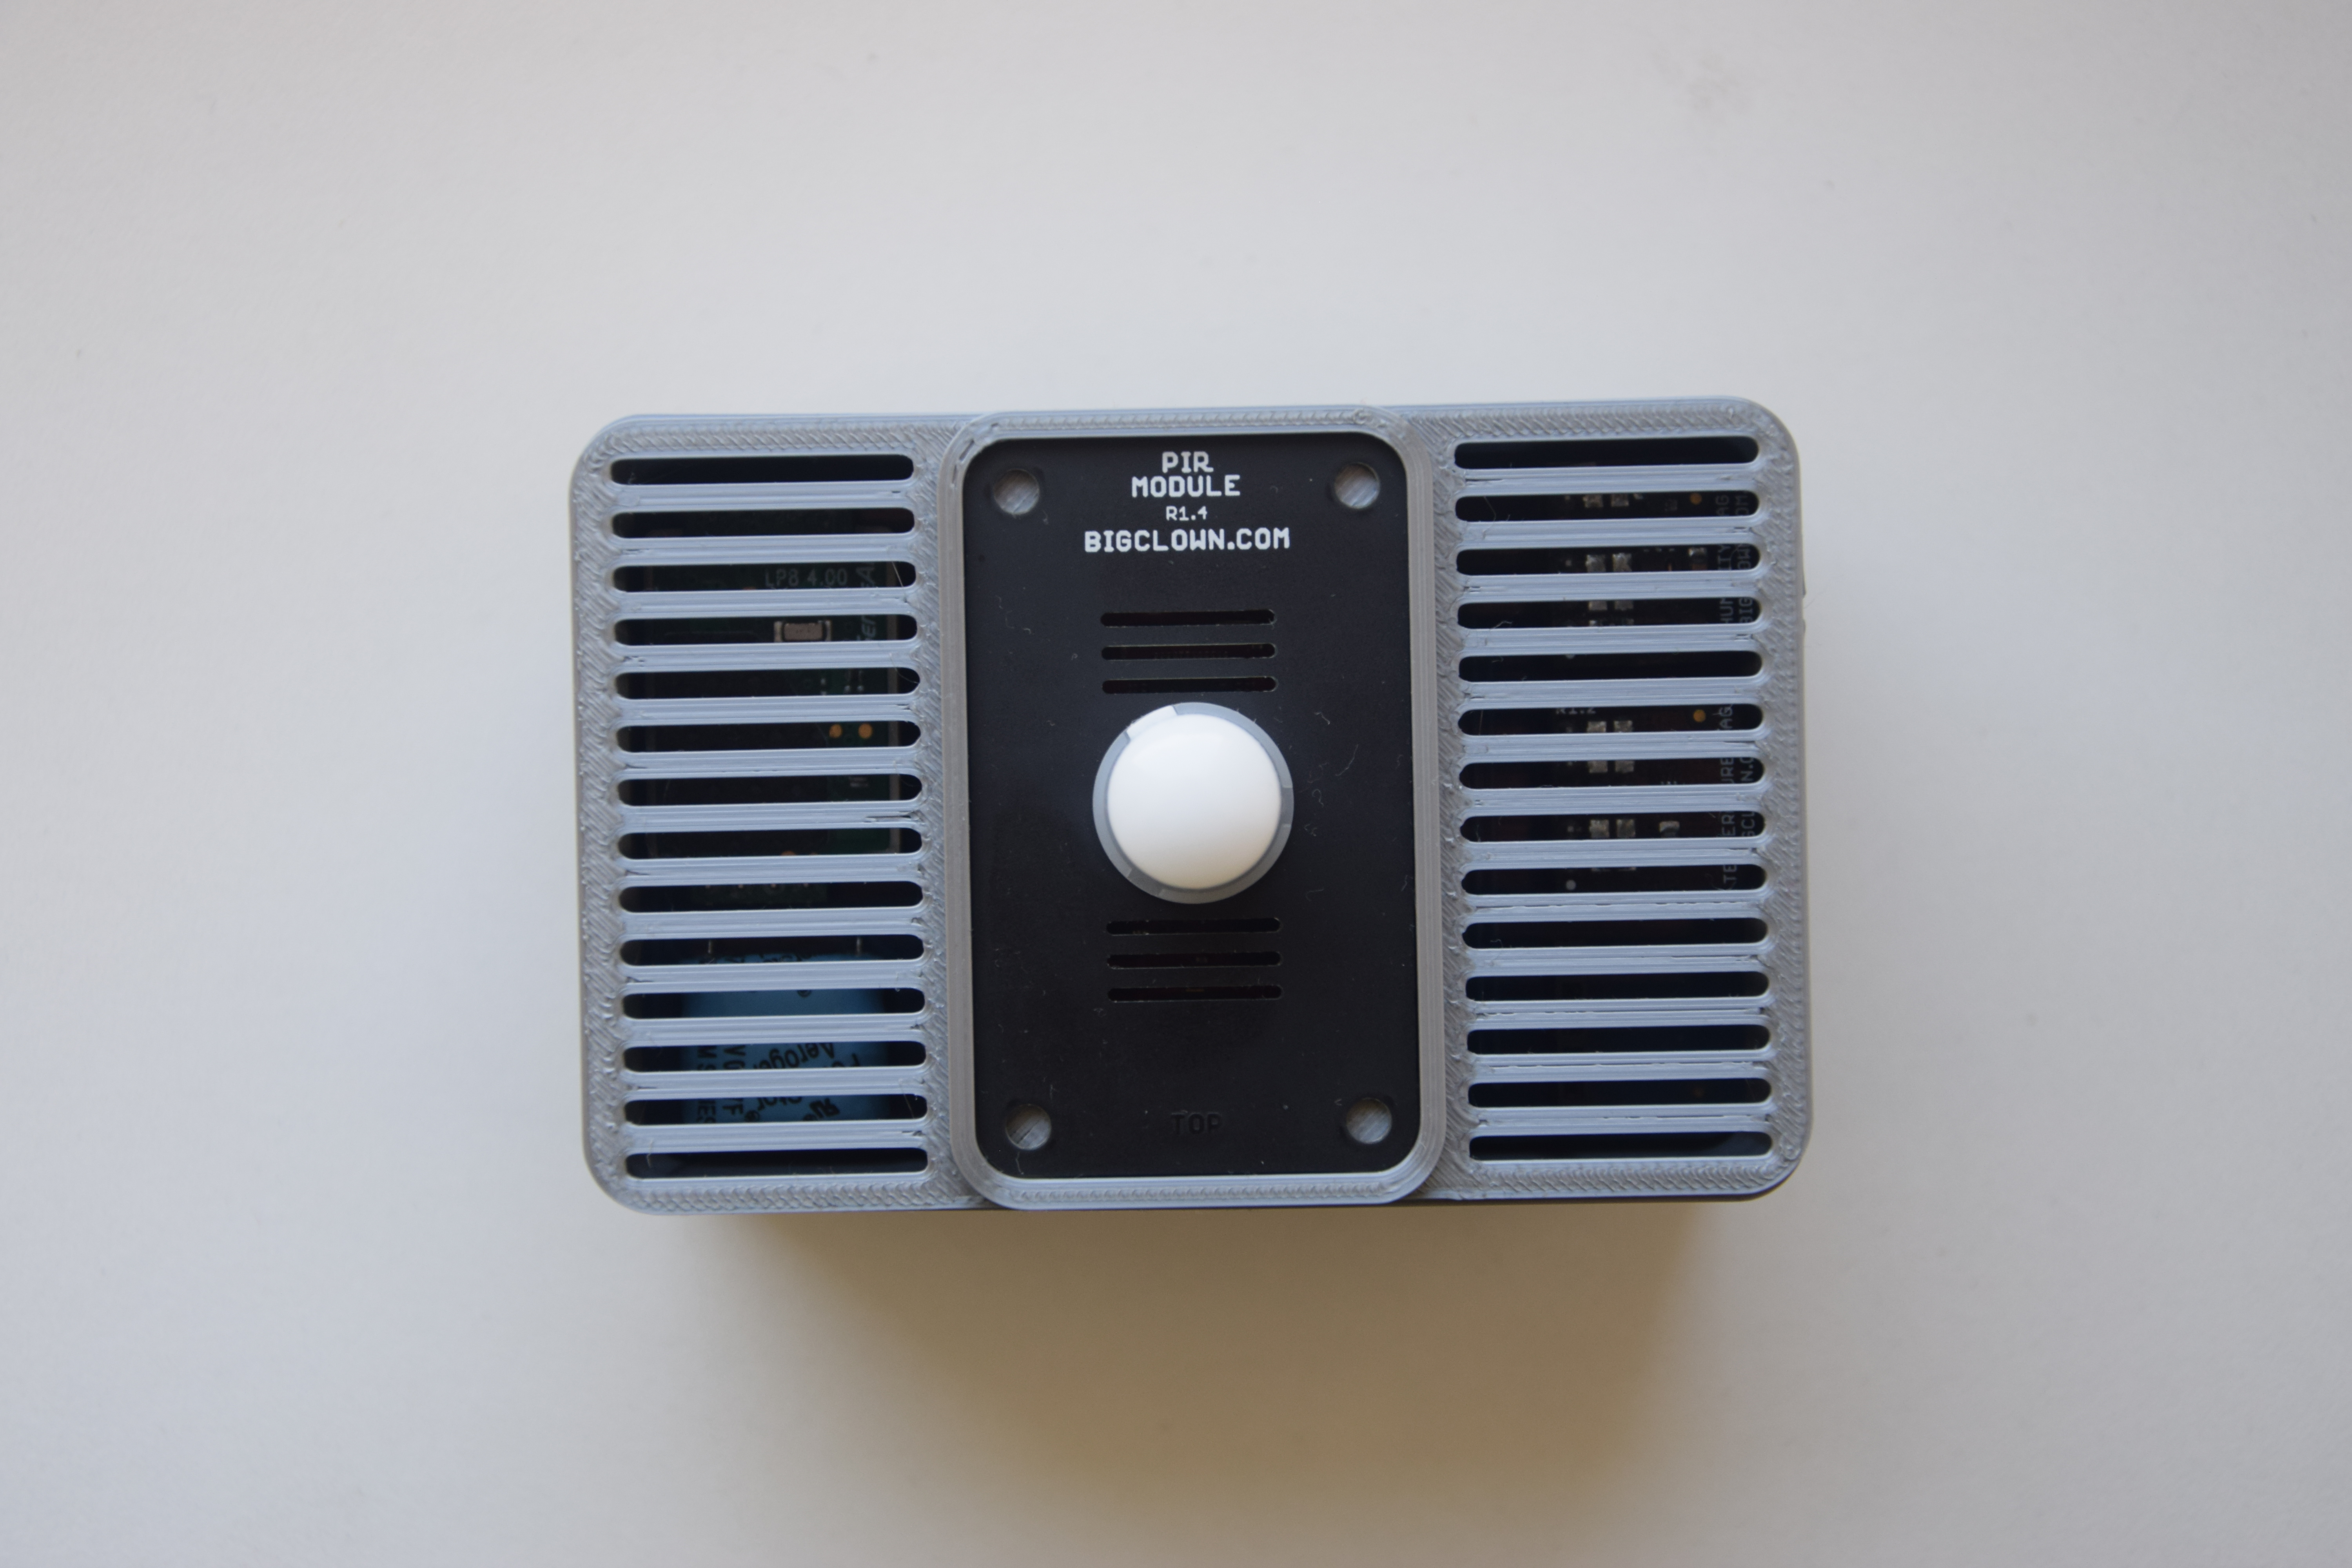
\includegraphics[width=\textwidth]{obrazky-figures/hardwarePhotos/environmentalMonitorWithPIRComplete.JPG}
    \caption{Monitor klimatických podmínek pro indoor s~detektorem pohybu. Foto autor}
    \label{completeCO2Monitor}
  \end{minipage}
  \hfill
  \begin{minipage}[b]{0.4\textwidth}
    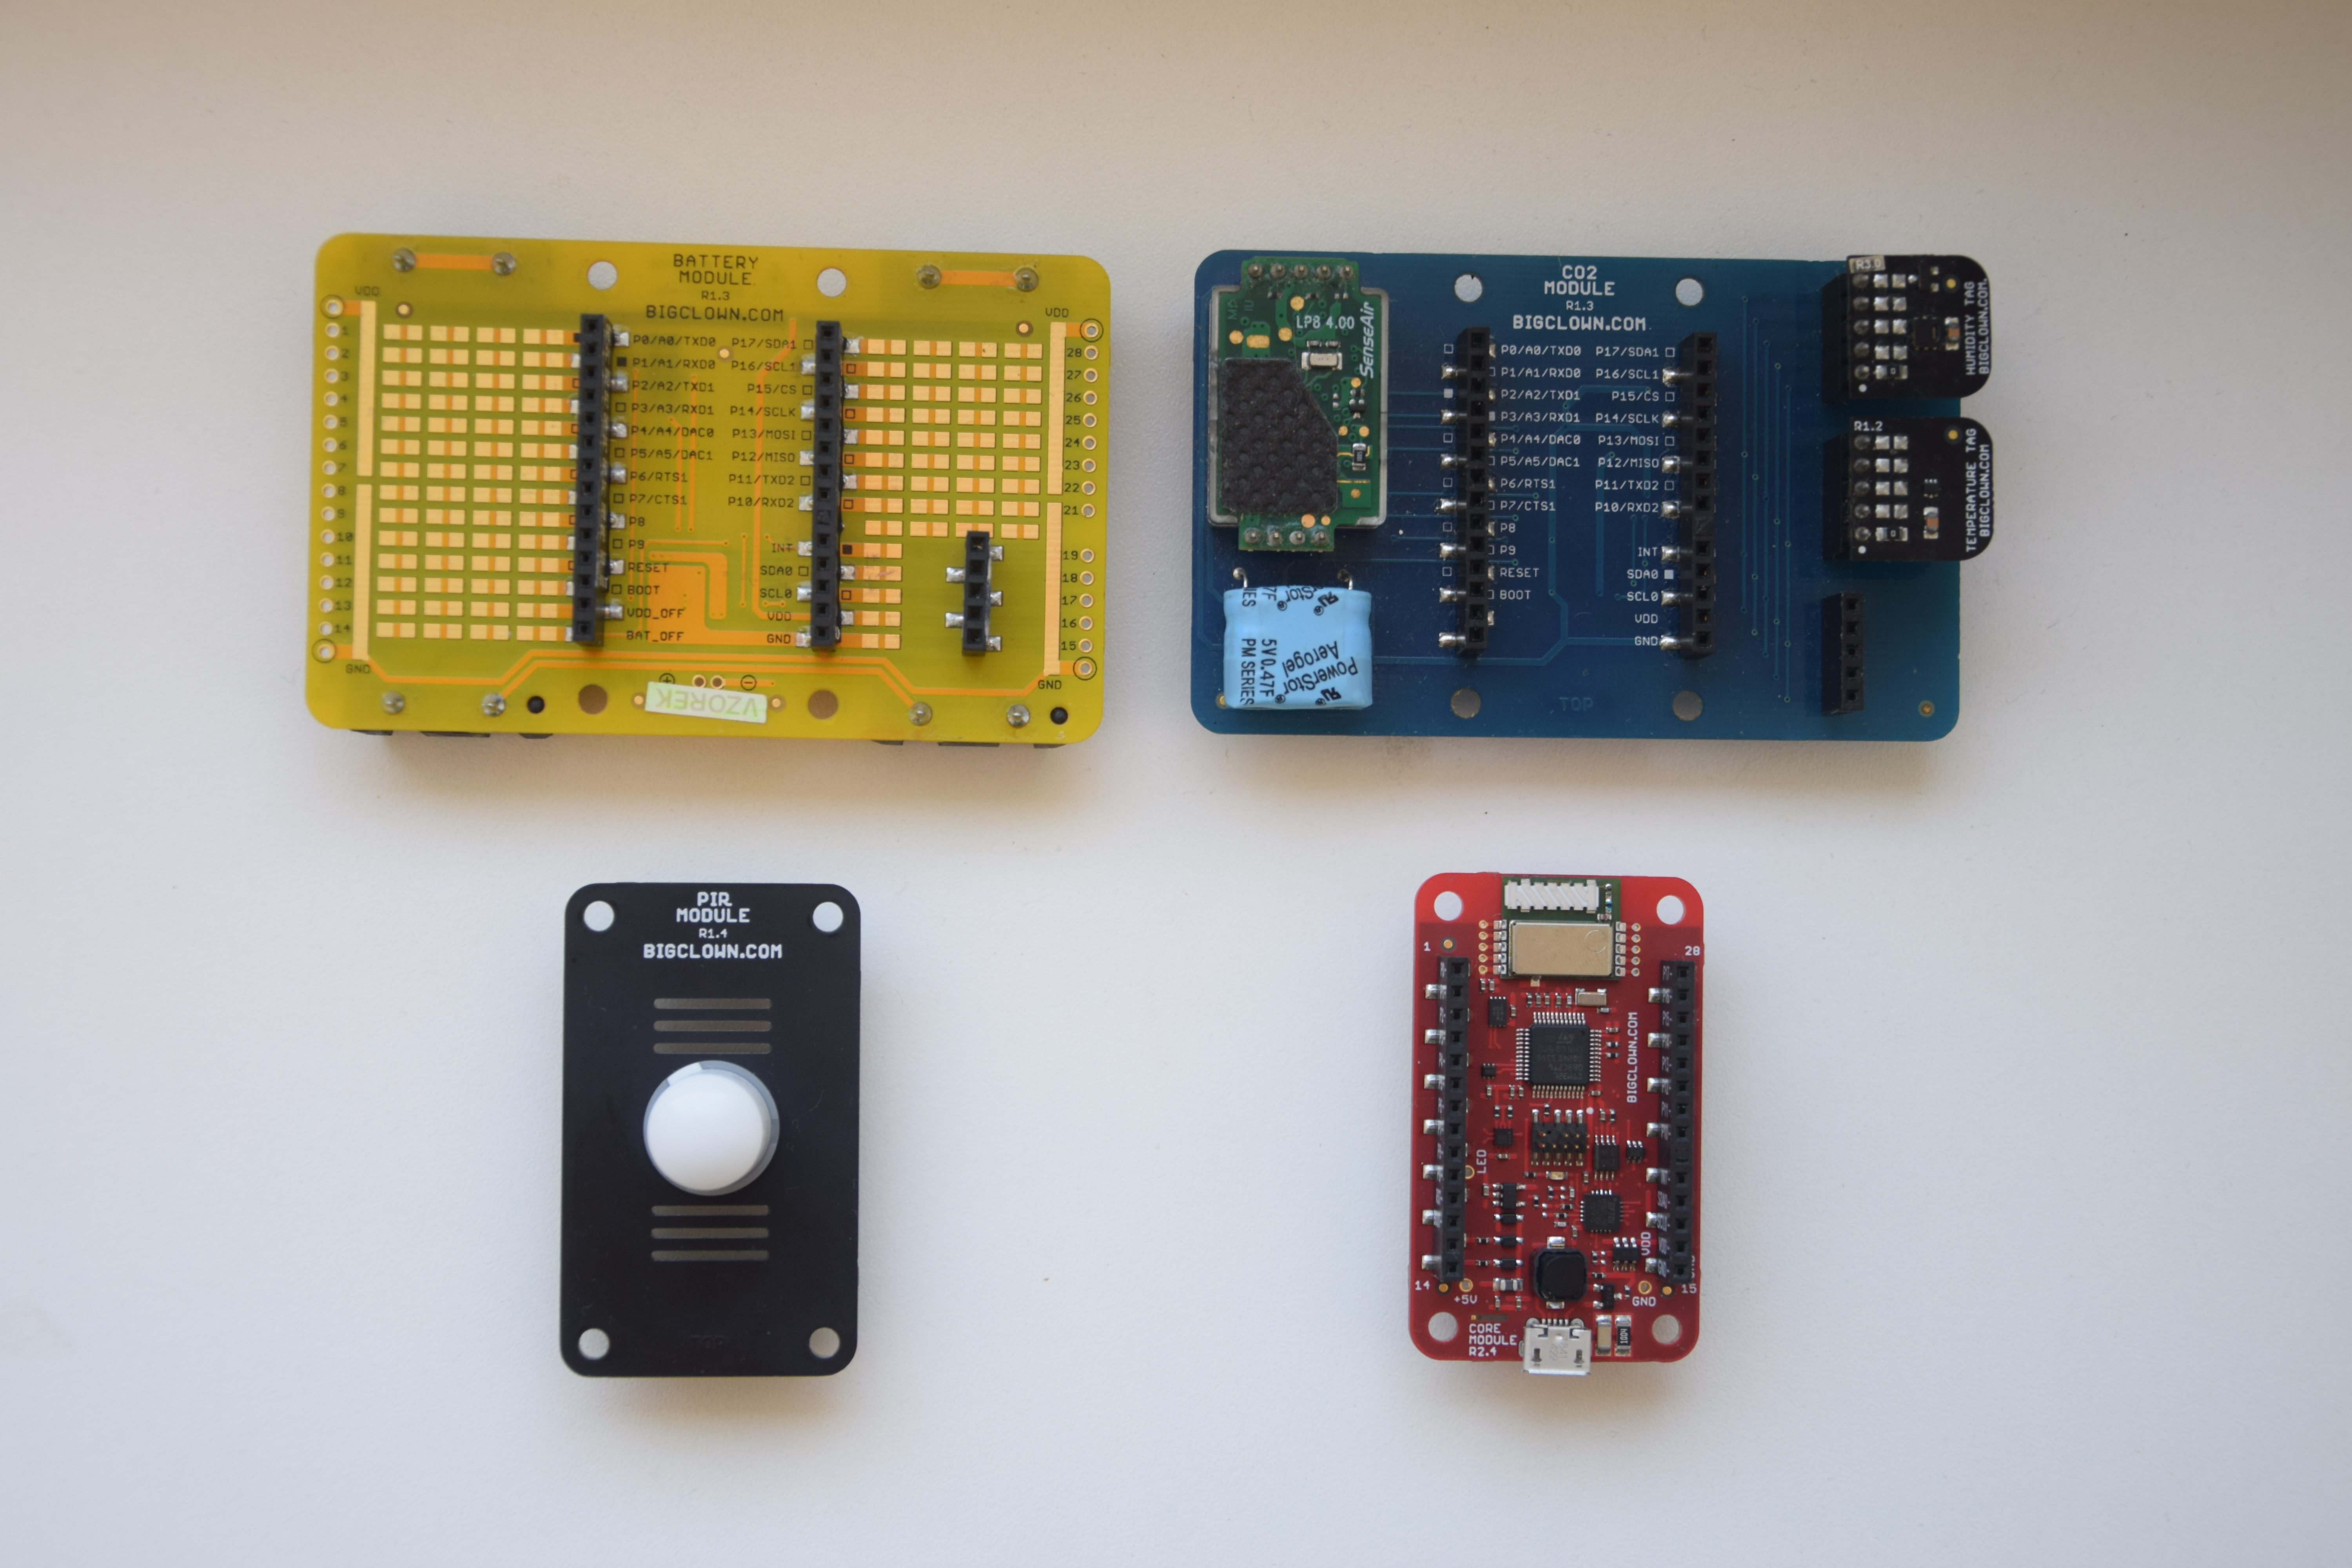
\includegraphics[width=\textwidth]{obrazky-figures/hardwarePhotos/environmentalMonitorWithPIRParts.JPG}
    \caption{Stejné zařízení rozložené na jednotlivé moduly. Foto autor}
    \label{disasembeledCO2Monitor}
  \end{minipage}
\end{figure}

Na obrázku \ref{disasembeledCO2Monitor} je vidět rozložené zařízení. Žlutý modul je napájecí bateriový modul, červený obsahuje samotný mikroprocesor a ovládá celé zařízení a černý modul se stará o~detekci pohybu pomocí PIR čidla. Modrý modul obsahuje měřič $CO_2$ a několik takzvaných tagů pro měření dalších klimatických podmínek. Složené zařízení ve vytisknuté krabičce je možné vidět na Obrázku \ref{completeCO2Monitor}.

\begin{figure}[H]
  \centering
  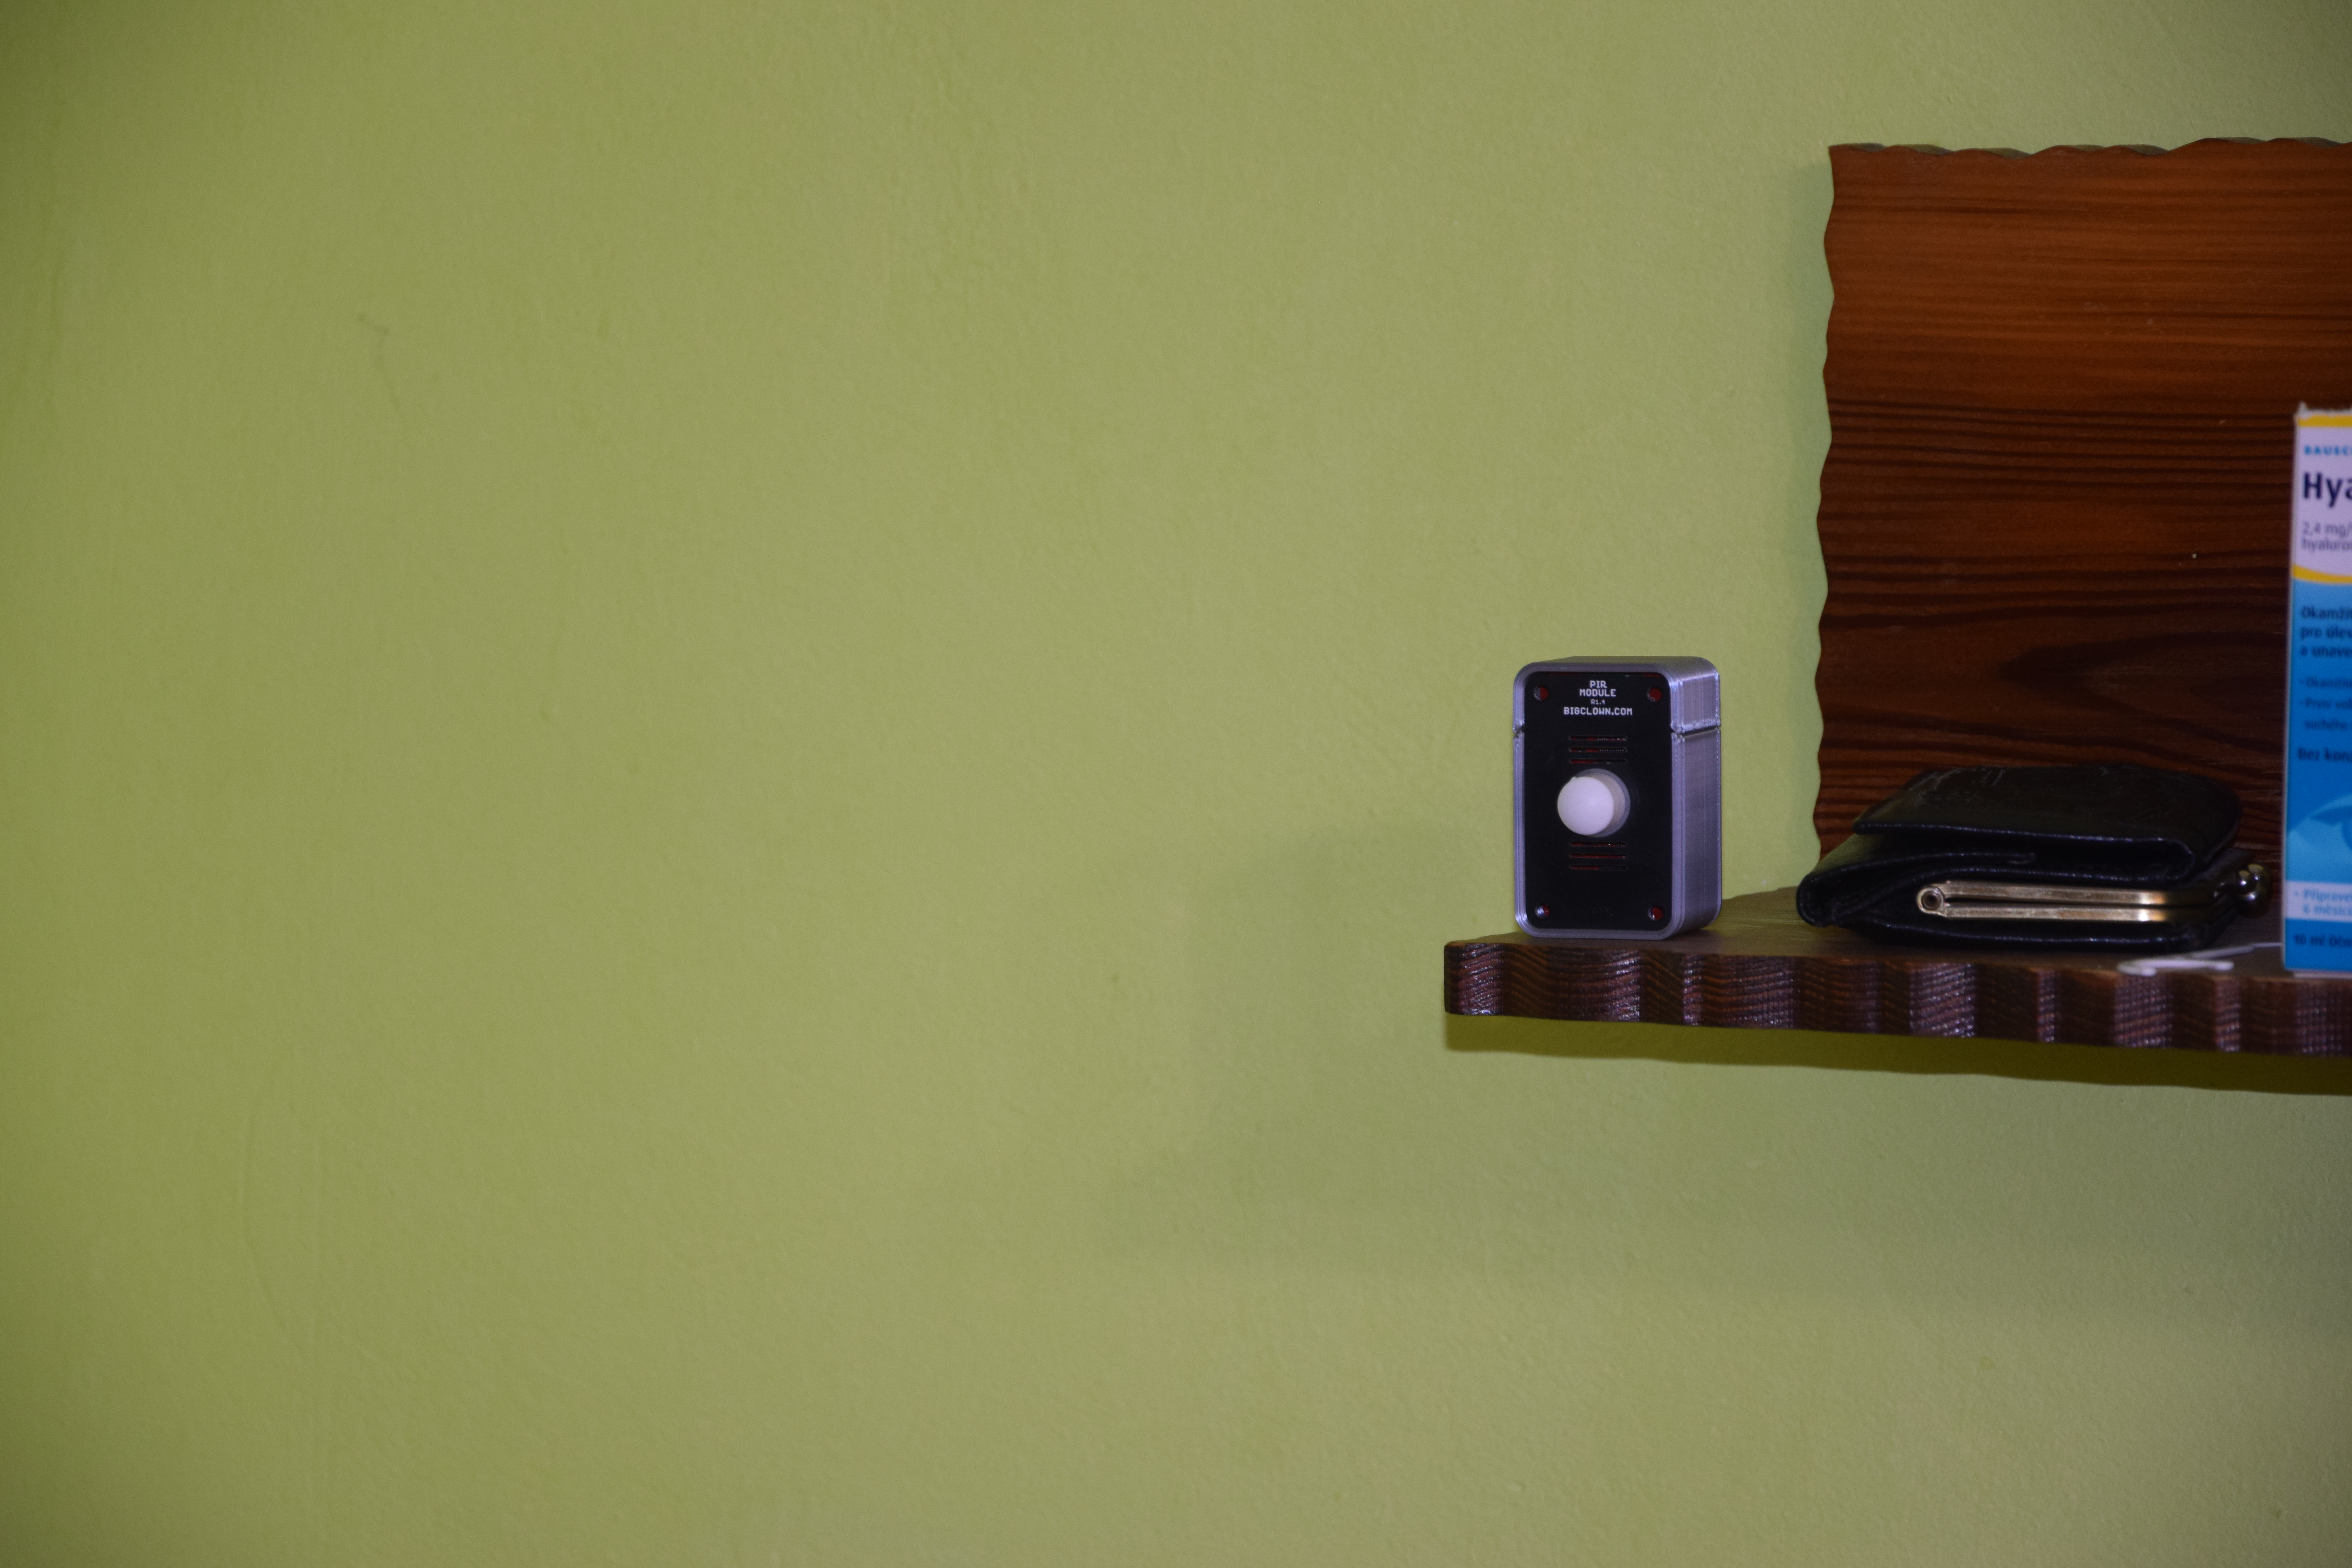
\includegraphics[width=\textwidth]{obrazky-figures/hardwarePhotos/placementShowcase.JPG}
  \caption{Ukázka umístění hardwarového zařízení v~domě. Foto autor}
  \label{placementShowcase}
\end{figure}

Na Obrázku \ref{placementShowcase} je možné vidět ukázku umístění jednoho z~vytvořených hardwarových zařízení. DAlší zařízení jako monitor CO2 či klimatických podmínek mohou být umístěna podobně. Zařízení s~PIR čidlem by měla být umístěna tak aby pokrývyla většinu místnosti.